% this file is called up by thesis.tex
% content in this file will be fed into the main document

%: ----------------------- name of chapter  -------------------------
\chapter{Analiza problemu integracji} % top level followed by section, subsection


%: ----------------------- paths to graphics ------------------------

% change according to folder and file names
\ifpdf
    \graphicspath{{4/figures/PNG/}{4/figures/PDF/}{4/figures/}}
\else
    \graphicspath{{4/figures/EPS/}{4/figures/}}
\fi

%: ----------------------- contents from here ------------------------


W tym rozdziale przanalizujemy przedstawione w poprzednim rozdziale przykładowe systemy pod kątem wyznaczenia części wspólnej, co pozwoli nam na uproszczenie i przyspieszenie implementacji tych systemów. W pierwszej części przedyskutujemy wymagania stawiane tym systemom, które z nich są ogólnymi wymaganiami aplikacji wykorzystujących synteze mowy, a które są szczególnymi wymaganiami danej aplikacji. W kolejnej części przedstawimy możliwe rozwiązania, przeanalizujemy je pod względem spełniania postawionych wymagań, a także przedstawimy wady i zalety każdego z nich.

\section {Analiza wymagań}

\section {Analiza dostępnych silników syntezy mowy}

Jako, że celem naszej pracy nie jest stworzenie własnego syntezatora mowy, lecz stworzenie systemów, które to będą wykorzystywać syntezatory mowy w celu implementacji swojej logiki biznesowej, kolejnym krokiem jest analiza dostępnych na rynku rozwiązań. 

Dostępne syntezatory są charakteryzowane przez następujące cechy:
\begin{itemize}
	\item sposób dostępu
	\item ilość obsługiwanych języków
	\item jakość generowanego dźwięku
	\item cena
	\begin{itemize}
		\item koszty początkowe(cena zakupu)
		\item koszty użytkowania (opłata za każde użycie)
	\end{itemize}
	\item perspektywy rozwoju
	\item łatwość użycia
\end{itemize}

Większość z tych cech jest jasna i nie wymaga dalszego opisu. Jedyną cechą która nie dokońca przemawia za siebie jest sposób dostępu. Sposób dostępu określa w jaki sposób możemy uzywać danego syntezatora, można powiedzieć, że definiuję interfejs jaki dany syntezator posiada. Pod względem sposobu dostępu, syntezatory mowy dzielimy następująco:

\begin{itemize}
	\item syntezatory zintegrowane  - rozwiązania wbudowane w urządzenię, pozawalające na synteze tylko we wcześniej przewdizianych przez producenta scenariuszach - 
		\begin{itemize}
			\item  Amazon Kindle
			\item  PocketBook eReader Pro
		\end{itemize}
	\item syntezatory stacjonarne - rozwiązania pozwalające na generację dźwięku w obrębie jednego urządzenia, zazwyczaj dostępne jako odrębne aplikacje lub biblioteki
		\begin{itemize}
			\item Festival Speech Synthesis System
			\item FreeTTS
			\item Loquendo Mobile
			\item Loquendo Multimedia
			\item Android TTS
		\end{itemize}
	\item syntezatory serwerowe - gotowe rozwiązania serwerowe, wykorzystujące specjalistyczne protokoły w celu zwiększenia wydajności 
		\begin{itemize}
			\item IVONA Telecom
			\item IVONA Speech Server
			\item Loquendo Speech Server
		\end{itemize}
	\item sytezatory SaaS
		\begin{itemize}
			\item IVONA Speech Cloud
		\end{itemize}
\end{itemize}

Sposób dostępu jednoznacznie wyznacza stopień trudności integracji syntezatora w środowisku SOA. Na początku listy znajdują się silniki syntezy mowy, które ciężko zastosować do tworzenia rozbudowanych systemów(rozwiązania zintegrowane), natomiast na końcu rozwiązania który z łatwością można wykorzystać do budowanie wszelakiego rodzaju systemów (rozwiązania SaaS).

Podjęcię decyzji, którego syntezatora będziemy używać, jak każda inna decyzja dotycząca architekury systemu, nie jest łatwa. Dodatkowo, zdecydowanie sie na jedno rozwiązanie bardzo często wymusi na nas wykorzystanie konkretnych technologii (np IVONA Telecom > MRCP), a także może nas pozbawić możliwości zmiany decyzji w przyszłości (przez brak standardów, wymiana jednego rozwiązania na inne moze wymagać dużego nakładu pracy).

\section {Architektura}

Znając wymagania które muszą spełniać przedstawione systemy, a także dostępne możliwości jeżeli chodzi o silniki syntezy mowy,  mozemy przejść do projektowania architektóry tych systemów.

%: ##################### AUTONOMICZNE SYSTEMY #########################################
\subsection {Autonomiczne systemy}
Pierwszym proponowanym podejściem jest podejście polegające na stworzeniu wyspecjalizowanych autonomicznych systemów dla każdego problemu z osobna. Na pierwszy rzut oka, podejście to jest sprzeczne z tematem pracy, ponieważ nie występuje w nim żadna integracja. Jednak po spojrzeniu na problem z perspektywy systemu wykorzystującego multimedia - systemy wykorzystujące synteze mowy zaliczają sie do tego typu systemów - podejście to jaka najbardziej trzeba poddać rozważeniu.

Systemy multimedialne charakteryzują sie specjalnymi wymaganiami w porównaniu do reszty systemów. Najważniejsze z nich to jak najmniejsze opuźnienie. Opuźnienia maja bardzo duży wpływ na to jak uzytkownicy odbierają daną aplikacje system. Weźmy na przykład system telekonferencji. Duże opuźnienia w takim systemnie nie tyle utrudniają co praktycznie uniemożliwiają korzystanie z takiego system. Pierwszy stopień opóźnień w prowadza sieć internet w której to takie systemy działaj. Czas propagacji sygnału, przepustowość sieci - wszystkie te cechy wpływają na opuźnienie. Z powodu wysokiego stopnia złożoności systemy te same z siebie wprowadzają pewien dodatkowy stopień opuźnień. U źródła danych zazwyczaj następuję kopresja danych i kodowanie do odpowniedniego formatu. Po drodze do użytkownika końcowego może nastąpić transkodowanie z jednego formatu na drugi, nawet wielokrotnie. Na końcu, u uzytkownika końcowego, następuje proces dekodowania i dekompresji. Każdy z tych procesów czy to u źródła danych , czy u użytkownika końcowego wymaga poświęcenia odpowiedniej ilości czasu. 

Z wyżej wymienionych powodów, ważne jest aby w systemach multimedialnych nie wprowadzać dodatkowych, niepotrzebnych opóźnien, a także, żeby nie zwiększać objętości danych. Podejście autonomicznych systemów pozwala nam na używanie specjalistycznych rozwiązań, które to pomogą nam osiągnać nasz cel biznesowy, a tażke spełnienie wymagań stawianych systemom multimedialnym. W podejściu tym, część odpowiadająca za logike biznesową oraz silnik syntezy mowy stanowią jeden autonomiczny system. Bardzo często działają one na jednym wspólnym urządzeniu, badź we wspólnej sieci wewnętrznej, dzięki czemu komunikacją miedzy nimi jest szybka i mniej zawodna. Komunikacja zachodzi bezpośrednio między wymienionymi składnikami systemu, bez zadnych elementów pośrednich. Dodatkowo rozwiązanie takie pozwla w pełni wykorzystać specyfike danej aplikacji, np aplikacja na telefon może używać wbudowanych silników syntezy mowy, dzięki czemu nie jest uzaleźniona od dostępu do internetu - oczywiście  kosztem jakości generowanego dźwięku. 


Wadą takiego rozwiązania jest nakład pracy potrzebny do stworzenia wszystkich systemów. Każdy system trzeba budować od podstaw. Wiedz zdobyta przy tworzeniu poprzednich systemów może okazać sie mało użyteczna, poniewać każdy system może być tworzony z myślą o innym silniku syntezy mowy,  z wykorzystaniem innych technologii. Kolejną wadą jest fakt że silnik mowy jest częścią systemu, przez co cały system jest mocno zaleźny od danego silnia. Jeżleli nagle nagle serwer syntezy mowy przestanie działać, cały system jest bezużyteczny. Problematyczna jest także wymiana silnika na inny. Przez mocne powiązanie podmiana silnika może wymagać dużego nakładu pracy. 

Ważna kwestią do przemyslenia, podczas projektowania jest też kwestia rozbudowy systemu. Dotychczas poruszaliśmy tylko temat sytezy mowy,  jednak jeżeli myślimy o stworzeniu w pełni wartościowego produktu, musimy zastanowić sie nad rozszerzeniem naszego systemu o dodatkową funkcjonalność taką jak:

\begin{itemize}
	\item autentykacja
	\item autoryzacja
	\item cachowanie
	\item księgowanie
	\item monitoring
\end{itemize}

Jeżeli uznamy, że nasze systemy potrzebują którejś z wymienionych funkcjonalności mamy do wyboru dwa wyjścia implementacje tych funckjonalności od zera, albo skorzystanie z gotowych, dostępnych usłgu dostarczających takich funkcjonalności. Wypisane wyżej funkcjonalności są same w sobie dość złożonymi problemami wymagajacymi dużych nakładów pracy, dlatego lepiej odrazu skupić sie na dostępnych usługach, które to są wykorzstywane przez wielu użytkowników, przez co mozemy być bardziej pewnie co do poprawności ich działania. Przy podejściu utonomicznych systemów, będzeimy musili osobno zintegrować każdy system, z usługami których on wymaga. I tak przy założeniu, że tworzymy \begin{math}n\end{math} systemów, i kazdy z nich będzie korzystał z \begin{math}m\end{math} usług to liczba połączeń system-usługa, które musimy stworzyć wynosi \begin{math}n*m\end{math}. Jak widać ilość pracy rośnie liniowo wraz z liczbą systemów i wraz z liczbą usług którtych te systemy chciały by wykorzystywać.

 Przykładową architekturę w w tym podejściu dla tworzonych systemów przedstawia rysunek \ref{fig:autonomiczne_systemy}

\setlength\fboxsep{20pt}
\setlength\fboxrule{1pt}
\begin{figure}[!h]
	\centering
	\fbox{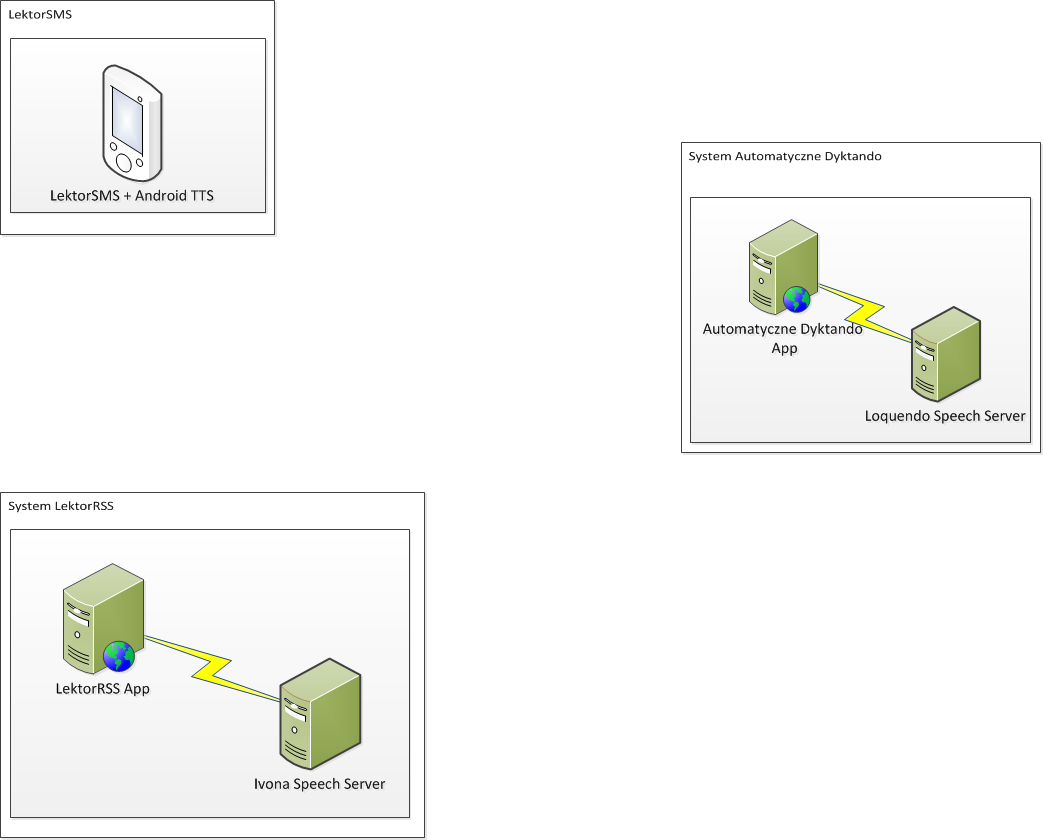
\includegraphics[scale=0.45]{wyspecjalizowane_rozwiazania.png} }
	\caption{Architekrura - Autonomiczne systemy}\label{fig:autonomiczne_systemy}
\end{figure}

Podejście autonomicznych aplikacji jest  skupione na konkretnych systemach, a nie na intergracji ich w istniejącym środowisku. Można nawet powiedzieć, że w tym podejściu w ogóle nie występuje element integracji. Jednakże, rozwiązanie to ma też swoje plusy. Przy tym podejściu, powstające systemy są lepiej dostosowane do stawianych przed nimi zadań, ale też wymagają wiekszych nakładów pracy i są cieżkie w rozbudowie. Kolejne podejście, które zostanie zaprezentowane  patrzy na problem z troche innej perspektywy. Nie jest oneaż tak  skupione na tworzonych systemach, lecz na ich współistnieniu z współpracy wraz z innymi systemami w środowisku SOA.

%: ##################### HUB and Spoke #########################################
\subsection {Podejscie zorientowane na usługi}
Dzięki postępowi technologicznemu przepustowość łączy internetowych wciąż wzrasta, dzięki temu to co pare lat temu było nie osiągalne dzis jest normą. Powstają nowe rodzaje usług, które kiedyś nie mogły by zostać zrealizowane, przy tworzeniu zaś niektórych aplikacji, to co kiedyś było problemem i na czym skupiali swój wysiłek twórcy oprogramowania, dzisiaj schodzi na drugi plan. Z drugiej jednak strony zwiększają sie wymagania użytkowników co do jakości multimediów, są wprowadzane coraz to nowe formaty, który wymagają ogromnych przepustowość. Czasami jednak systemy mulitmedialne nie mają takich scisłych wymagań co do wielkości opóźnienia. W ich przypadku opóźnienie nawet rzędu kilkudziesięciu sekund nie stanowi problemu i jest akceptowalny przez użytkowników. W takim wypadku nie trzeba sie skupiać na szukaniu idealnego rozwiązania dla danego problemu, lecz można sie skupić na stworzeniu architektóry która ułatwi i przyspieszy budowanie systemów zpełniających dane wymagania.

Przy takim podejściu do tworzenia systemu zazwyczaj pojawia sie problem integracji budowanego systemu z istniejącymi już usługami. Często też, budowany system jest całkowicie problemem integracyjnym, czyli wszystkie składowe usługi potrzebne do realizacji celu biznesowego są dostępne, a jedyne zadanie stawiane budowanemu systemowi to opdowiednia integracja tych usług. Podejście takie ułatwia parę kwesti, ale w zamian wprowadza także nowe, specyficzne dla siebie problemy. Głownym problememe jest różnorodność dostępnych podsystemów. Każdy z nich może być stworzony przy użyciu innych technologii (Java, COM, .Net, CORBA, ICE, itp.) działać na innej platformie (MS WINDOWS, LINUX, SOLARIS) i co najważniejsze mogą wykorzystywać inne protokoły do komunikacji (RPC, SOAP, własnościowe protokoły, itp). Z tego powodu decyzja o podejsiu integracyjnym nie powinna być podejmowana zbyt pochopnie i powinna być podjęta bazując na pewnych kryteriach. Przykładowe kryteria:  \cite{hohpewoolf2003} 

\begin{itemize}
	\item \textbf{powiązanie aplikacji} - integracja aplikacji powinna minimalizować powiązania i zależności między nimi, co pozwoli na swobodne rozwijanie każdej aplikacji z osobna. Sciśle powiązane aplikacje współdziałają przy wielu założeniach z każdej ze stron. Jeżeli któraś z aplikacji zostanie zmieniona i założenia co do niej nie będą już spełnione wtedy cała integracja przestanie działać. Dlatego też, projektowane interfejsy powinny być na tyle specyficzne aby umożliwiały implementacje użytecznych funkcjonalności, lecz także na tyle ogólne aby umożliwiały zmiane implementacji, jeżeli zajdzie taka potrzeba.
	\item \textbf{poziom ingerencji} - podczas integracji aplikacji, powinno się minimalizować zarówno zmiany w samej aplikacji jak i ilość kodu tworzonego na rzecz integracji. Jednak bardzo często zarówno zmiany w aplikacji jak i tworzenie dodatkowe kodu odpowiadającego za integracje jest nie uniknione aby uzyskać odpowiednią funkcjonalność. Rozwiązania mniej ingerujące w aplikacje mogą nie zapewniać integracji w odpowiednim stopniu.
	\item \textbf{wybór technologii} - do wyboru mamy mnóstwo technologii integracyjnych, które różnią się od siebie wymaganiami co do specjalistycznego sprzętu i do oprogramowania. Nie które z nich są wymienne między sobą, natomiast wybranie innych może prowadzić na zamknięcie sie na dane rozwiązanie. Jeżeli podejmie sie decyzje o zastosowaniu którejś z gotowych technologii integracji może ona znacząco zwiększyć koszt całego system. Z drugiej strony, integracja od podstaw zazwyczaj kończy się wiekszym nakładem pracy niż początkowo planowano i może oznaczać odkrywanie koła na nowo.
	\item \textbf{format danych} - integrowane aplikacje muszą posługiwać sie tym samym formatem podczas wymiany danych. Dostosowywanie istniejących aplikacji do jednolitego formatu danych może być bardzo trudne, albo wręcz nie możliwe. Inną opcją jest wprowadzenie elementu pośredniego, którego celem będzie tłumaczenie danych z jednego formatu na drugi. Problemem powiązanym z opisanym w tym podpunkcie jest problem rozszerzalność i rozwój formatu danych - jak format danych może sie zmieniać z biegiem czasu i jak te zmiany wpłyną na aplikacje.
	\item \textbf{żywotność danych} - integracja powinna minimalizować czas pomiędzy udąstępnieniem danych przez jedną aplikację, o pobraniem tych danych przez drugą aplikacje. Można to osiągnąć poprzez częstą wymianę małych porcji danych, jednakże takie podejście moze zmniejszyć wydajność całego systemu. Opuźnienia związane z wymiąną daynch muszą zostać wzięte pod uwagę podczas planowania integracji. W idealnym systemie, aplikacja odbiorca zostanie poinformowana jak tylko dane będą dostępne. Im dłuższy czas miedzy publikacja a konsumpcją danych tym większa szansa, że aplikacje ulegną rozsynchronizowaniu.
	\item \textbf{rodzaj komunikacji} - przetwarzanie komputerowe jest w dużej większości synchroniczne - to znaczy, że jedna procedura wywołuje drugą ( podprocedurę) i czeką na jej wykonanie. W systemach rozproszonych, wywołania mają charakter zdalny, co powoduję, że są o wiele wolniejsze od wywołań lokalnych. Z tego powodu, oczekiwanie na zakończenie wywołania, jest często nie porządane. W takim wypadku można wykorzystać podejście asynchroniczne - prrocedura wywołują podprocedurę, lecz nie czeka na jej zakończenie jak to było w wypadku wywołania synchronicznego, tylko wraca do swojego przetwarzania. Kiedy podpprocedura zakończy przetwarzanie, informuję o tym procedurę wywołująca i zwraca jej wynik. Komunikacja asynchroniczna może zwiększyć wydajność całego systemu, ale również moze uczynić go bardziej złożonym.
	\item \textbf{poziom niezawodności} - komunikacja zdalna jest nie tylko wolniejsza, ale również bardziej zawodna niż lokalne wywołania funkcji. Kiedy procedura wywołują podprocedurę w obrębie jednej aplikacji, jest pewne, że ta podprocedura jest dostępna. Takie założenie nie musi być spełnione jeżeli chodzi o zdalne wywołania - zdalna aplikacja moze nie działać w chwili wywołania, albo połączenie z siecią może być chwilowo niedostępne.
\end{itemize}



ksiazka ESB strony 4,5 

opiszemy to podejscie i potem opiszemy, ze jest bardzo fajne, opiszemy rodzaje, jak ewoluowało, i na koncu opiszemy esb, a potem konkrety dla naszej aplikacji. Obrazki w ksiazce ESB
ESB strona 34 - czemu własnościowe rozwiązania sa do dupy 



\subsection {Szyna} 

Przedstawienie jak to wyglada( kropki serwisy , komunikują sie z roznymi innymi serwisami, dodatokwe serisy: accounting itd)

Wymagania stawiane rozwiazaniom integracyjnym , Czy warto integrować ? (book1.pdf chapter 2)

Integracja systemow multimedialnych ??

Rozwiazania ?

Brak integracji

integracja EAI - hub and spikes (scentralizowany punk, single point of failure. słabo scalowalne)

SOA - ESB 




service activator (request od clienta)


% ---------------------------------------------------------------------------
%: ----------------------- end of thesis sub-document ------------------------
% ---------------------------------------------------------------------------

